\documentclass[12pt]{article}
\usepackage[paperwidth=8.5in,paperheight=11in,margin=1in]{geometry}
\usepackage{float}
\usepackage{lipsum}
\usepackage{parskip}
\usepackage{bbding}
\usepackage{amssymb}
\usepackage{titlesec} 
\usepackage{graphicx}
\usepackage{hyperref}
\usepackage{setspace}
\usepackage[section]{placeins}
\newcommand{\tline}{\hspace{-2.3pt}$\bullet$ \hspace{5pt}}
\hypersetup{colorlinks=true, linkcolor=black, urlcolor=blue}
\setlength{\parindent}{15pt} % Indent paragraphs (automatically)

\makeatother
\makeatletter
\setlength{\@fptop}{0pt}

\begin{document}
	\begin{titlepage}
		\centering	
		\vspace{1cm}
  
		{\scshape\Large CS 383: Software Engineering Semester Project\par}
    \begin{figure}[h]
      \centering
      
\includegraphics[width=0.7\linewidth]{uislogan}
    \end{figure}   
		\vspace{2.5cm}
    
		{\huge\bfseries Goofy Lights Design Specification\par}
		\vspace{2cm}	
    
		{ \setstretch{0.1}		
  		{\Large\itshape Adrian Beehner\par}
  		{\Large\itshape Andrew Butler\par}
  		{\Large\itshape Seth Forrest\par}
  		{\Large\itshape Joseph Leister\par}
  		{\Large\itshape Animesh Pattanayak\par}
  		{\Large\itshape Megan Phelan\par}
  		{\Large\itshape Robert Stewert\par}		
		}		
    \vspace{1.5cm}	
    
		supervised by\par
		Bruce Bolden		
		\vfill		
		% Bottom of the page
		{\large \today\par}
	\end{titlepage}

	\tableofcontents
	\newpage
	
	\section{Introduction}
		\subsection{Project Summary}
  		The University of Idaho Marching Band has recently begun an experimental project to place glasses on members of the band that light up according to a specified design. The task described in this document is part of a semester project for the Software Engineering class (CS 383) at the University of Idaho and is to design and implement a graphical user interface (GUI) for this project, known colloquially as \textit{Goofy Lights}. This GUI should grant a user the ability to manipulate the state and color of each node to create elaborate designs and patterns. This piece of software should be intuitive enough that it will be usable by any individual with little or no training. The program should allow a user to manipulate the color and state of a single node, multiple nodes, or bulk properties of all nodes. The workspace should allow the layout of greater than the actual number of nodes required by the customer. In addition, the user should be able to specify workspace dimensions. This software will be written in Java.
		
		\subsection{Document Purpose}
  		This document is a design specification for a Software Engineering (CS 383) semester project at the University of Idaho. The purpose of this document is to outline the approach and initial design of this project. It will define terms used, specific design choices, and provide a rudimentary time-line of project goals. 
		
		\subsection{Definition of Terms}
		\begin{itemize}
			\item Node - An individual pair of GoofyGlasses
			\item GoofyGlasses - A pair of glasses with RGB LEDs in them and a wireless receiver that are programmed to light up specific colors. Using this grid editor the glasses can be placed in array and light up in specific patterns or can be synced to music.
			\item IDE - Integrated Development Environment, a tool used to write and develop a software program.
			\item GUI - Pronounced "gooey" the Graphical User Interface is the front end of a program that the user interacts with.
			\item WYSIWYG - Pronounced "whizzy wig" this acronym stands for What You See Is What You Get. It is often associated with graphical tools that allow you to drag and drop objects in order to design a GUI, web-page, or other graphical output. 			
		\end{itemize}
		
		\subsubsection{Java JDK}
  		This program will be written in Java, requiring use of the Java Development Kit (JDK). At the time of this document the current release is version 8 update 121 and can be downloaded from Oracle at \url{http://www.oracle.com/technetwork/java/javase/downloads/jdk8-downloads-2133151.html}
		
		\subsubsection{Swing}
  		Swing is a set of libraries that can be imported into Java programs in order to create a rich GUI experience without having to import all the classes and methods for the GUI individually. While there is no specific download for the Java's swing package the following Javadoc is helpful in identifying the different classes/components that can be used. \url{https://docs.oracle.com/javase/8/docs/api/javax/swing/package-summary.html}
		
		\subsubsection{Eclipse}
  		Eclipse is a Java based IDE that allows for easy code development. It helps keeps files organized and has some built in debugging capabilities. Eclipse is used widely in the community and thus offers many options for third party plug-ins to assist in development. More information along with downloads of the latest version of Eclipse can be found at \url{https://eclipse.org/}
		
		\subsubsection{WindowBuilder Pro}
  		WindowBuilder Pro (\url{https://eclipse.org/windowbuilder/download.php}) is a plug-in for Eclipse that makes GUI design quicker and easier than coding from scratch. This plug-in adds a 'design' tab to Eclipse's interface that adds tools for clean WYSIWYG design. 
		
\newpage
	\section{Program Overview/Scope}
  	This software is being developed with scalability in mind. The goal is to create a Framework that can be updated and scaled easily, and to some degree, efficiently. Changes in the development cycle will require adding the basic framework(the editor itself) and various functionalities, such as different sets of editors(single vs. multiple node). This program will have a GUI that allows manipulation of the color and state of each node, multiple nodes simultaneously, or bulk manipulation of the entire array. Grid dimensions and number of nodes should be variable(yet reside at a default value unless the user specifies). It will be assumed that no nodes in the grid are allowed to change places, all nodes must reside in their original location relative to other nodes. Another assumption is that the glasses themselves are already setup with a \textit{n}-node channel receiver, being able to receive $3$-byte message-for RGB values. The program will be able to run on any Operating System with Java installed, with no changes in functionality, each OS will utilize its own specific file system properties when loading and saving configurations.
	
	%----------------------------------------------------------------------------------------
	%	COMPONENT OVERVIEW
	%----------------------------------------------------------------------------------------
	\subsection {Component Overview}
  	There are seven main components in the system software; Configuration Editor, Single Node Editor, Multi-Node Editor, Grid Editor, Character Editor, Animation Creator, and File Generator. The Configuration Menu Bar will provide a simple interface for setting up and/or configuring the grid of glasses, in addition to saving and loading a project. The Single Node Editor will provide the user with an interface to edit individual Nodes. The Multi-Node Editor will provide the user with an interface to edit multiple( possibly all) Nodes. The Grid Editor will provide the user with an interface to edit a scalable grid that contains space larger or smaller than the current specified/default amount of nodes. The Character Editor will provide the user with an interface for editing, creating, and saving of any special grid formations, with default numbers and letters preloaded. The Animation Creator will allow the user to create animations with characters from the Character Editor, allowing the user to create animations via corresponding grid(s). The File Generator is a simple interface that allows the text representation of the animations created in the Animation Creator to be a saved to a \textit{tan} file format. A diagram showing user interaction with the 4 basic components (Configuration Editor, Single Node Editor, Multi-Node Editor, and Grid Editor) is shown in Figure 1.	
  	\begin{figure}[ht!]
  		\centering
  		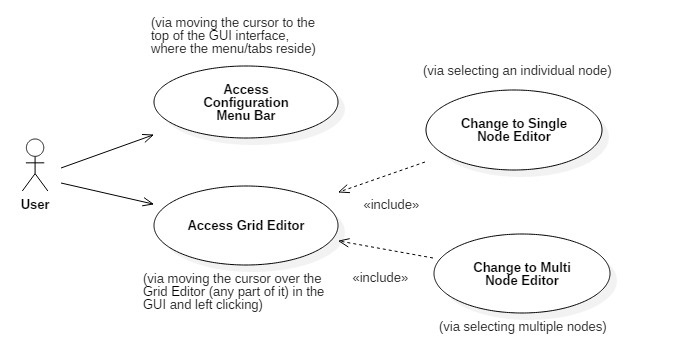
\includegraphics[width=\linewidth]{ComponetOverview.JPG}
  		\caption{Use Case Diagram of "Basic" Component Overview \label{overflow}}
  	\end{figure}
	
  
	%----------------------------------------------------------------------------------------
	%	CONFIGURATION
	%----------------------------------------------------------------------------------------
	\subsubsection {Configuration Menu Bar}
  	The configuration menu bar will provide a simple interface via a horizontal menu bar on the GUI that provides the user with various options on how they wish to configure the number of nodes; things like grid size, and status of a unit's connectivity. The number of nodes option will provide a simple dialog box to enter the number of nodes the user wishes to use and adjust the grid accordingly.  A dialog box will appear when the grid size option is accessed that will provide users the ability to select a dimension. Only grid dimensions will be allowed if all the $n$-nodes can fit within that space, otherwise an error will be displayed. In the file option/tab a user will be allowed to open a saved project, create a new project, save the current project, or 'save as' the current project. 
    The only input accepted is from clicking on a tab to access it's dialog boxes and displays. This menu bar has controls for how the dimensions of the grid editor components are laid out, and does have dependencies that it relies on to function properly. There are some system resource demands for the tasks in this menu, such as registering the number of nodes, changing the grid dimensions, and pairing glasses. These can all become resource intensive if the number of nodes is large enough, and overhead due to GUI demands can occur. The general use-case of this component is shown in Figure 2.	
  	\begin{figure}[ht!]
  		\centering
  		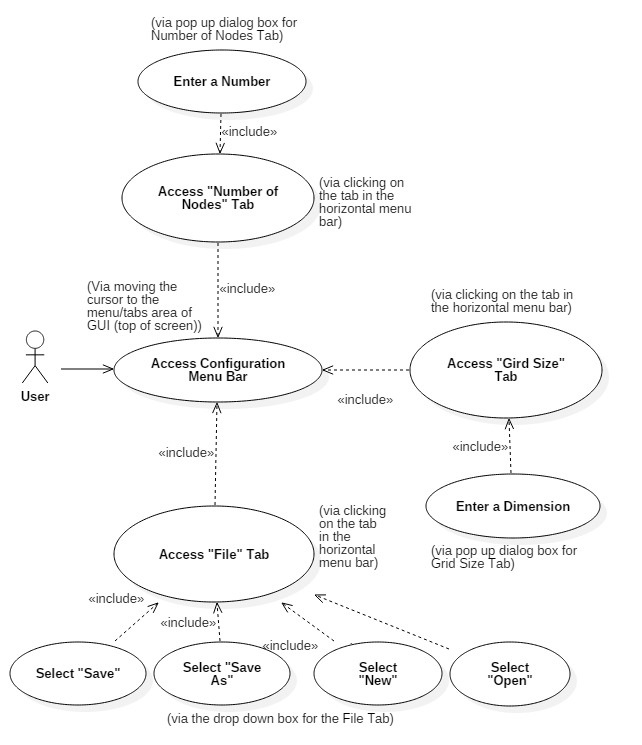
\includegraphics[width=\linewidth]{Configuration_Editor.JPG}
  		\caption{Use Case Diagram of the Configuration Menu Bar \label{overflow}}
  	\end{figure}
	
	%----------------------------------------------------------------------------------------
	%	SINGLE NODE EDITOR
	%----------------------------------------------------------------------------------------
	\subsubsection {Single Node Editor}
  	The Single Node Editor in the system software will allow the user to edit any individual node via a user interface. This means the user can hand pick various nodes and set specific colors to them. Thus the component allows users to edit any individual node on the grid, choose a color via dialog box, and see the feedback via Grid Editor. The only inputs are from clicking on the individual node-grid node and then click on a color via the dialog box. Outputs are displaying the color dialog box, the node-grid node with the chosen color, and eventually a signal to the glasses. This component is dependent on the Grid Editor to display the nodes and provide an interface. Constraints of this program are that it cannot be changed from this mode when editing a node is in process, and thus no other actions (in the system software) may be performed while editing a node (or the component will actually exit editing the node without applying any changes). This task should not make an intensive use of system resources, however overhead may occur due to the GUI. The general use-case of this component can be seen below in Figure 3.  	
  	\begin{figure}[ht!]
  		\centering
  		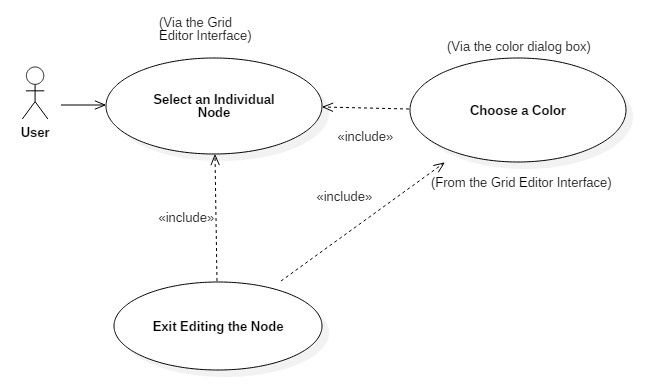
\includegraphics[width=\linewidth]{SingleNodeEditorDiagram.JPG}
  		\caption{Use Case Diagram of Single Node Editor \label{overflow}}
  	\end{figure}
  
	\begin{figure}[ht!]
    \centering
    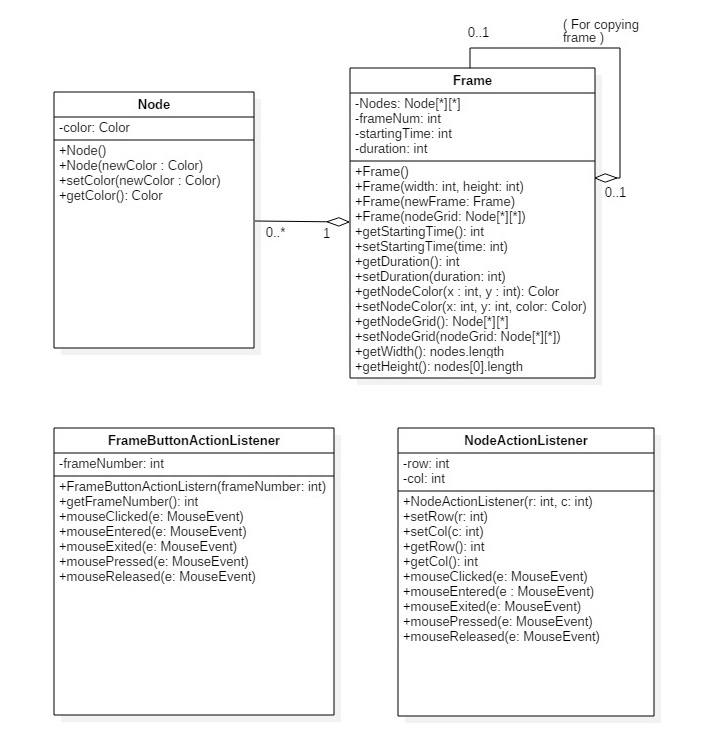
\includegraphics[width=0.9\linewidth]{Class_Diagram_Frame_Node_and_ActionListener_Classes.JPG}
    \caption{Diagram for Frame, Node, FrameButtonActionListener, and NodeActionListener Classes}
  \end{figure}
	
	%----------------------------------------------------------------------------------------
	%	MULTI NODE EDITOR
	%----------------------------------------------------------------------------------------
	\subsubsection {Multi-Node Editor}
  	The Multi-Node Editor component is in charge of editing all the nodes within a grid. This component handles the selection of individual or multiple nodes. For example, the user may want to select a 20x20 sub-grid and change the color to green. The Multi-Node Editor is responsible for allowing the user to select up to 400 nodes. 
    This selection should be done in a way that is familiar to the user. One possible action-sequence starts with the user selecting a node in a corner of the sub-grid. Then, while holding down shift, the user would select the node in a corner of the sub-grid diagonal to the first node selected. The Multi-Node Editor would be responsible to select all of the nodes in this sub-grid. The constraint being that this method will only select rectangular grids.	
  	After nodes are selected, the Multi-Node Editor should give the user an opportunity to edit the properties (like color or on/off status) via the Single Node Editor.   	
  	The Multi-Node Editor should also display a representation of the grid to the user via the GUI. See below for a mock-up of the selection of a 2x2 sub-grid within an 8x8 grid.
	
	%----------------------------------------------------------------------------------------
	%	GRID EDITOR
	%----------------------------------------------------------------------------------------
	\subsubsection {Grid Editor}
  	The Grid Editor is responsible for the creation, selection, and manipulation of grids. Since the goal of this program is to create visualizations with the nodes, it is paramount to allow the functionality to create and edit multiple grids. The grids work similar to a sprite animation; there is a collection of grids that will be cycled through in real-time with a slight delay. This can be used creatively to show animations.  	
  	In regards to creation, the Grid Editor must take user input to create a new grid( perhaps a '+' button) and assign corresponding data and GUI representations of the new grid. The user must also be able to delete grids. This component creates the ability to select single or multiple grids in a similar fashion to the Multi-Node Editor.  	
  	Additionally, the Grid Editor should allow the user to rearrange grids. This could take the form of dragging an individual grid to a different location within the grid array. Navigation of the various grids is necessary. The grid editor will implement this functionality, perhaps with a scroll bar (see figure below).	
    

  
  
  	\begin{figure}[ht!]
  		\centering
  		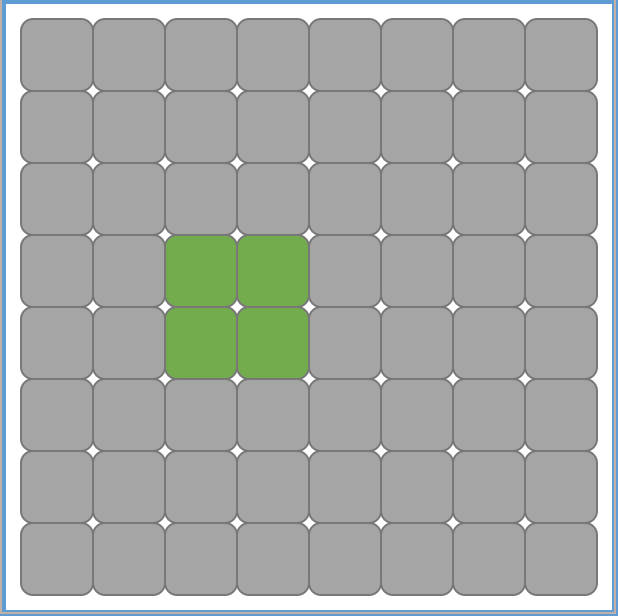
\includegraphics[width=80mm]{Grid.png}
  		\caption{Grid Selection (green nodes are selected)}
  	\end{figure}
  	
  	\begin{figure}[ht!]
  		\centering
  		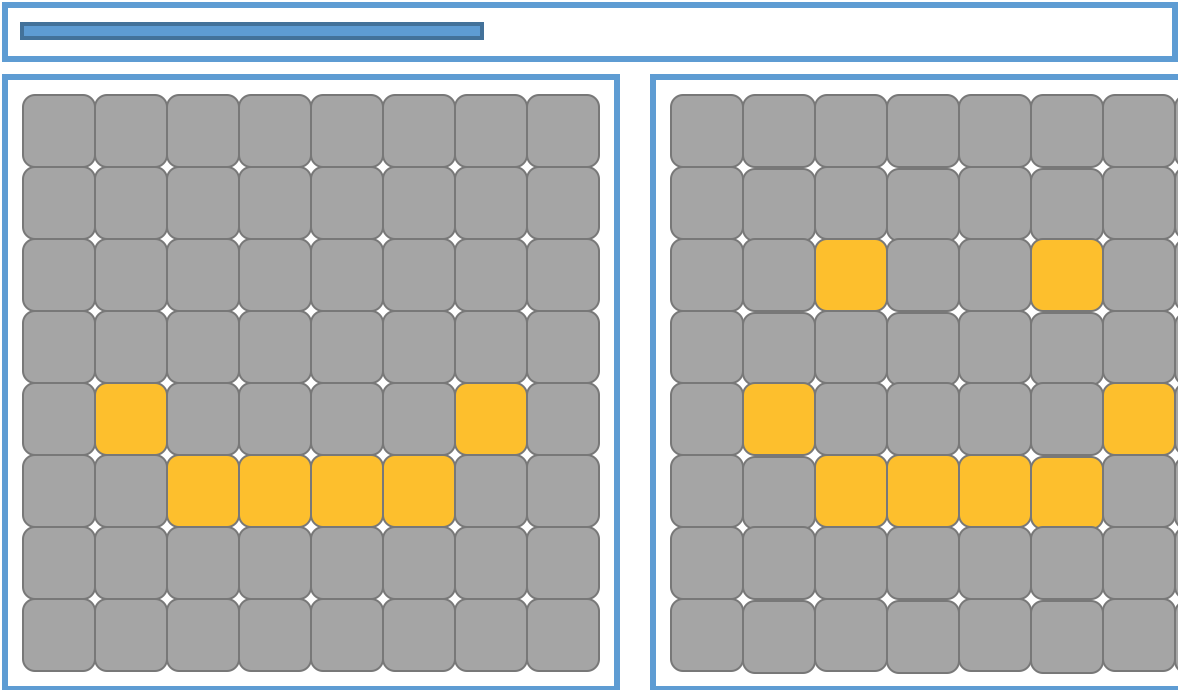
\includegraphics[width=100mm]{Multi-grid.png}
  		\caption{Multi-Node Grid Editor w/ Scroll Bar}
  	\end{figure}    
  
    \begin{figure}[ht!]
      \centering
      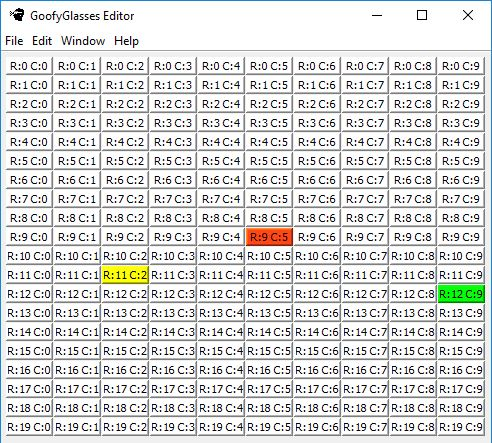
\includegraphics[width=150mm]{protoGrid.JPG}
      \caption{Grid Selection (The prototype of the grid editor)}
    \end{figure}
	\clearpage	
	
	%----------------------------------------------------------------------------------------
	%	Frame Preview Bar
	%----------------------------------------------------------------------------------------
	\subsubsection {Frame Preview Bar (Scrub Bar)}
	The Frame Preview Bar is responsible for the viewing and selection of frames (saved grid formations). It provides an interface that shows the user a simple "preview" of the current list of frames. By default the frame preview bar is blank until the user edits a node. Upon loading a TAN file, the frame preview bar will generate a list of frames that was read in. The Frame Preview Bar also works alongside "Add Frame (+)" button, which will take the current configuration of the grid and append that frame to the current frame list. The Frame Preview Bar will then update its graphic to reflect this change. The only inputs available are clicking upon the frame preview for the corresponding frame, which then will have the GUI load the frame's configuration into the grid editor. The other input is clicking and dragging the scroll bar (provided there is more frames than that can fit on the frame preview) to move through the list of frames. This preview bar has some system resource demands, as the actions described are resource intensive, such as having the frame preview bar generate a preview for each frame. An example of the Frame Preview Bar is shown in the following diagram.
	
	\begin{figure}[ht!]
		\centering
		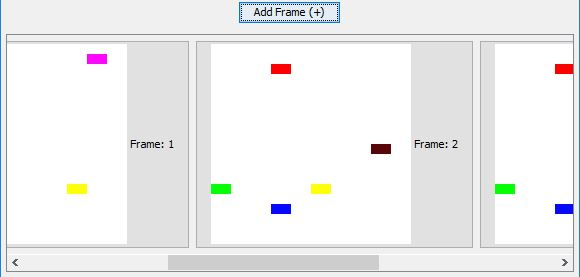
\includegraphics[width=150mm]{potoFramePre.JPG}
		\caption{Frame Preview Bar}
	\end{figure}

	
	%----------------------------------------------------------------------------------------
	%	 Character Editor
	%----------------------------------------------------------------------------------------
	\subsection { Character Editor}
  	The Character Editor is responsible for the creation, editing, loading, and saving of special grid formations, known as characters. By default, letters and numbers( perhaps other standard keyboard characters) should exist in the character editor. Each character, like the letter 'A', is assigned a corresponding grid that represents it.	
  	These default characters should be available regardless of grid size. The Character Editor allows the user to easily change a character's state, regardless of whether it is a default character or not.	
  	Additionally, the Character Editor should allow for the creation of new characters. For example, ':)' might be saved as 'smiley face'. These user-created characters are intrinsically tied to their corresponding grid size. These new characters must also be saved for future use.
	
	\subsubsection{Animation Creator}
  	The Animation Creator should implement the functionality to allow the user to create animations with characters. The Animation Creator should supply a text box for the user to input characters. The Animation Creator should then allow the user to pick an animation, like scrolling left to right, for the sequence of characters.	
  	Based off of this, the Animation Creator should generate corresponding grids that simulates the animation of the characters. The user, should be able to edit the generated grids with the other components. 
	
	\subsubsection{File Generator}
  	This component is responsible for outputting a text representation of the animations created in the program. The file must be in the "tan" format for use by the glasses and for future editing via this program.
	
	\subsubsection{Component Relationships}
  	The first component that the user will interact with is the Configuration Menu Bar. Setup steps, like setting grid size, will be taken from the user and initialize the other components.	
  	After setup, a default grid of size $n$ by $m$ (as specified by the user in the Configuration Menu Bar) is displayed. The Grid Editor is responsible for creating new grids and creating a Multi-Node Editor instance to manage every new grid. When a node is deleted via the Grid Editor, it is responsible to destroy the Multi-Node Editor for the deleted grid.  	
  	When the user selects one or multiple nodes and chooses to edit their properties, the Multi-Node Editor is responsible to call up the Node Editor. The Node Editor will then change the data representation of the edited node(s) which will then be reflected in the GUI as displayed by the Multi-Node Editor.  	
  	Alternatively, the user can use the Animation Creator to generate grids which can then be edited with the Grid Editor, Multi-Node Editor, or Node Editor. The Animation Editor uses characters available through the Character Editor.  	
  	See the use case diagram below.	
    
  	\begin{figure}[ht!]
  		\centering
  		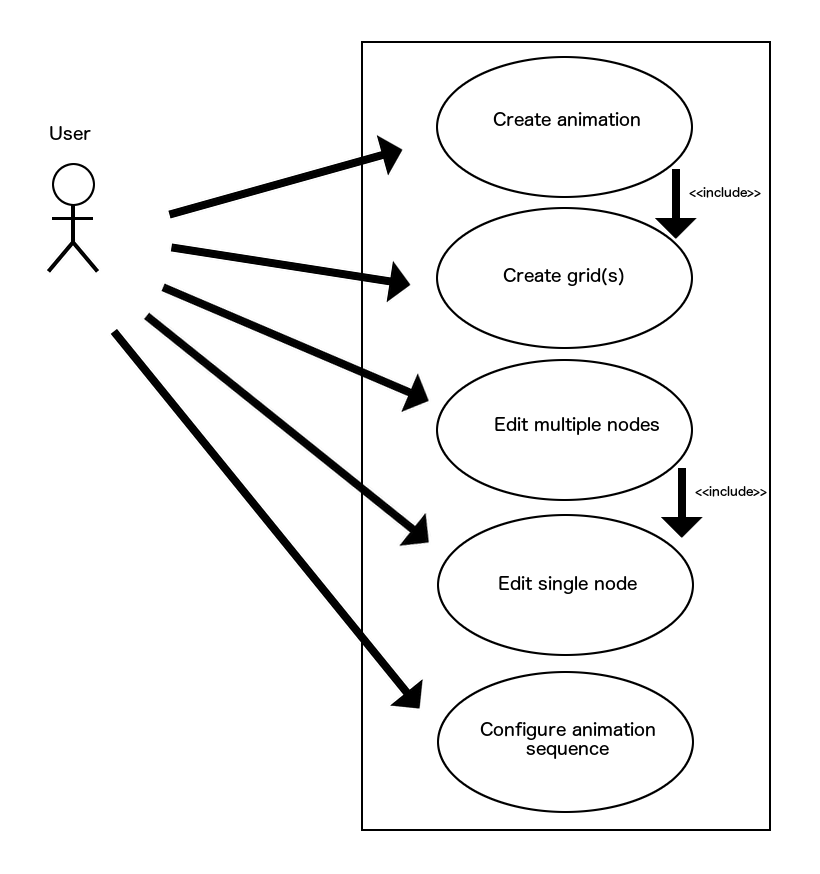
\includegraphics[width=0.9\linewidth]{Relationship_Use.png}
  		\caption{Use Cases}
  	\end{figure}
	\clearpage	
\newpage

	\section{Design Decisions}
    When planning this project, several decisions were made to limit the scope and complexity of the final product. These decisions are detailed below. 
    
  	\subsection{TAN File}
	  	The user is able to save and load TAN files via the GUI interface. A TAN file is a text file with the following format.
      The first line indicates the program version number. The next line specifies the name of an audio file(or states noAudioFile) which is to be loaded by the TAN player. The third line states the value in RGB for current state of color wheel. The fourth line lists the sixteen recently used RGB colors. The fifth line specifies the number of grids, then the next two values are the dimensions of the grid. Then starting with the sixth line, the TAN file begins the frames, with the first line of the "frame" stating the time (in milliseconds) the frame will appear. Then all the remaining lines represent each row, thus if the grid size was 3x3, there would three additional lines. Each line then has 3 * (the number of columns) of values, allowing for each node/cell having a RGB value corresponding to it. Going back the 3x3 example, having 3 * 3 (rows) = 9 values for each line, where 3 of those values are the RGB for one cell/node. Saving the current configuration of the frames from the GUI will convert the information into TAN file format, so the user can save and load files as often as needed. As mentioned before, TAN files can then be loaded, and then the GUI will load the information to display the new grid, changing the grid dimensions as specified by the file, and displaying the first frame.
  	
  	\subsection{Language Decisions}
    	Java is the primary tool used in this project. It is convenient as it works easily across platforms, is very readable, and provides its own graphics package. Swing is a graphics package designed to make APIs that work and look the same across all Java platforms. It is built into the language so no external libraries are needed. The use of Qt integration for Java, Qt Jambi, was considered but ultimately dismissed as that this would add complexity without providing functionality. 
      
  	\subsection{Constant Positions}
    	Each node must maintain a constant position relative to one-another. If the nodes are free to move around during a performance, and the software needed to support such moving, the complexity would increase drastically. Only by limiting the editor to a static configuration of nodes does this project become reasonable. 
      
  	\subsection{Grid Scalability}
    	The user will be able to set the grid dimensions to be used for the performance they are creating. In some cases, the editor will display a grid larger than the current number of nodes. In such a case the active nodes will be indicated. A solid rectangular grid will be the only supported configuration. The user will account for any unused nodes in the rectangle when designing characters or animations. Limiting the grid to a rectangle dramatically reduces the amount of options the editor needs to support, and there are few cases in which a non-rectangular array is desirable.
      
  	\subsection{Letters and Default Animations}
    	After viewing the Tower of Lights editor, it was decided that adding some default configurations to the editor would be convenient. These include static letters and built in animations such as animating characters from one end of the grid to another. Adding this functionality will significantly improve ease-of-use to the editor, while not adding insurmountable complexity to the project. 
      
\newpage
	\section{Timeline}

	{ \setstretch{2.0}		
  	\scalebox{1}{  		
  		\begin{tabular}{r |@{\tline} l}  			
  			March 6  & Design Specifications Version 1     \Checkmark              \\			
  			March 21 & Begin Sprint 1 of GoofyLights       \Checkmark              \\
        March 23 & Develop GUI for Single Node Editor  \Checkmark              \\
        March 25 & File I/O for Single Node            \Checkmark              \\
  			March 27 & Unit Testing for Sprint 1           \Checkmark              \\
        March 30 & End Sprint 1 and Begin Sprint 2     \Checkmark              \\
  			April 4  & File I/0 for GUI                    \Checkmark              \\
  			April 6  & Begin Development of Frame Editor   \Checkmark              \\
  			April 11 & End Sprint 2 and begin Sprint 3     \Checkmark              \\
  			April 13 & Complete Frame Editor                             \\
        April 16 & Complete Multi Node Editor                        \\
  			April 18 & Extra time to catch up or add additional features \\
  			April 20 & Goal Specifications for System Testing            \\
  			April 25 & System Testing                                    \\
  			May 1    & Preparation for Final Presentation                \\
  			May 4    & GoofyLights Final Presentation                    \\  			
  		\end{tabular}  		
  		}  	
	}

\end{document}
